\chapter{Techniques to Improve SDE/SPDE Inference}
\chaptertoc{}

\section{Presentation of Practical Challenges}

When acquiring any type of data, an experimentalist has to face two challenges among several others. The first is the time between two measurements, called the sampling time, which we would like to be as small as possible. However, many practical issues constrain the sampling time. As an example, fluorescent proteins used to image the biological object of interest lose their fluorescent properties when acquiring several different images. Thus, for fluorescent proteins, increasing the sampling time is particularly interesting for increasing the observation time. The second issue is the measurement error, defined as the difference between a measured value of a quantity and its unknown true value. Any measurement has its inherent measurement error. Thus, it is very important that any inference method is robust to measurement noise.

\begin{figure}
    \centering
    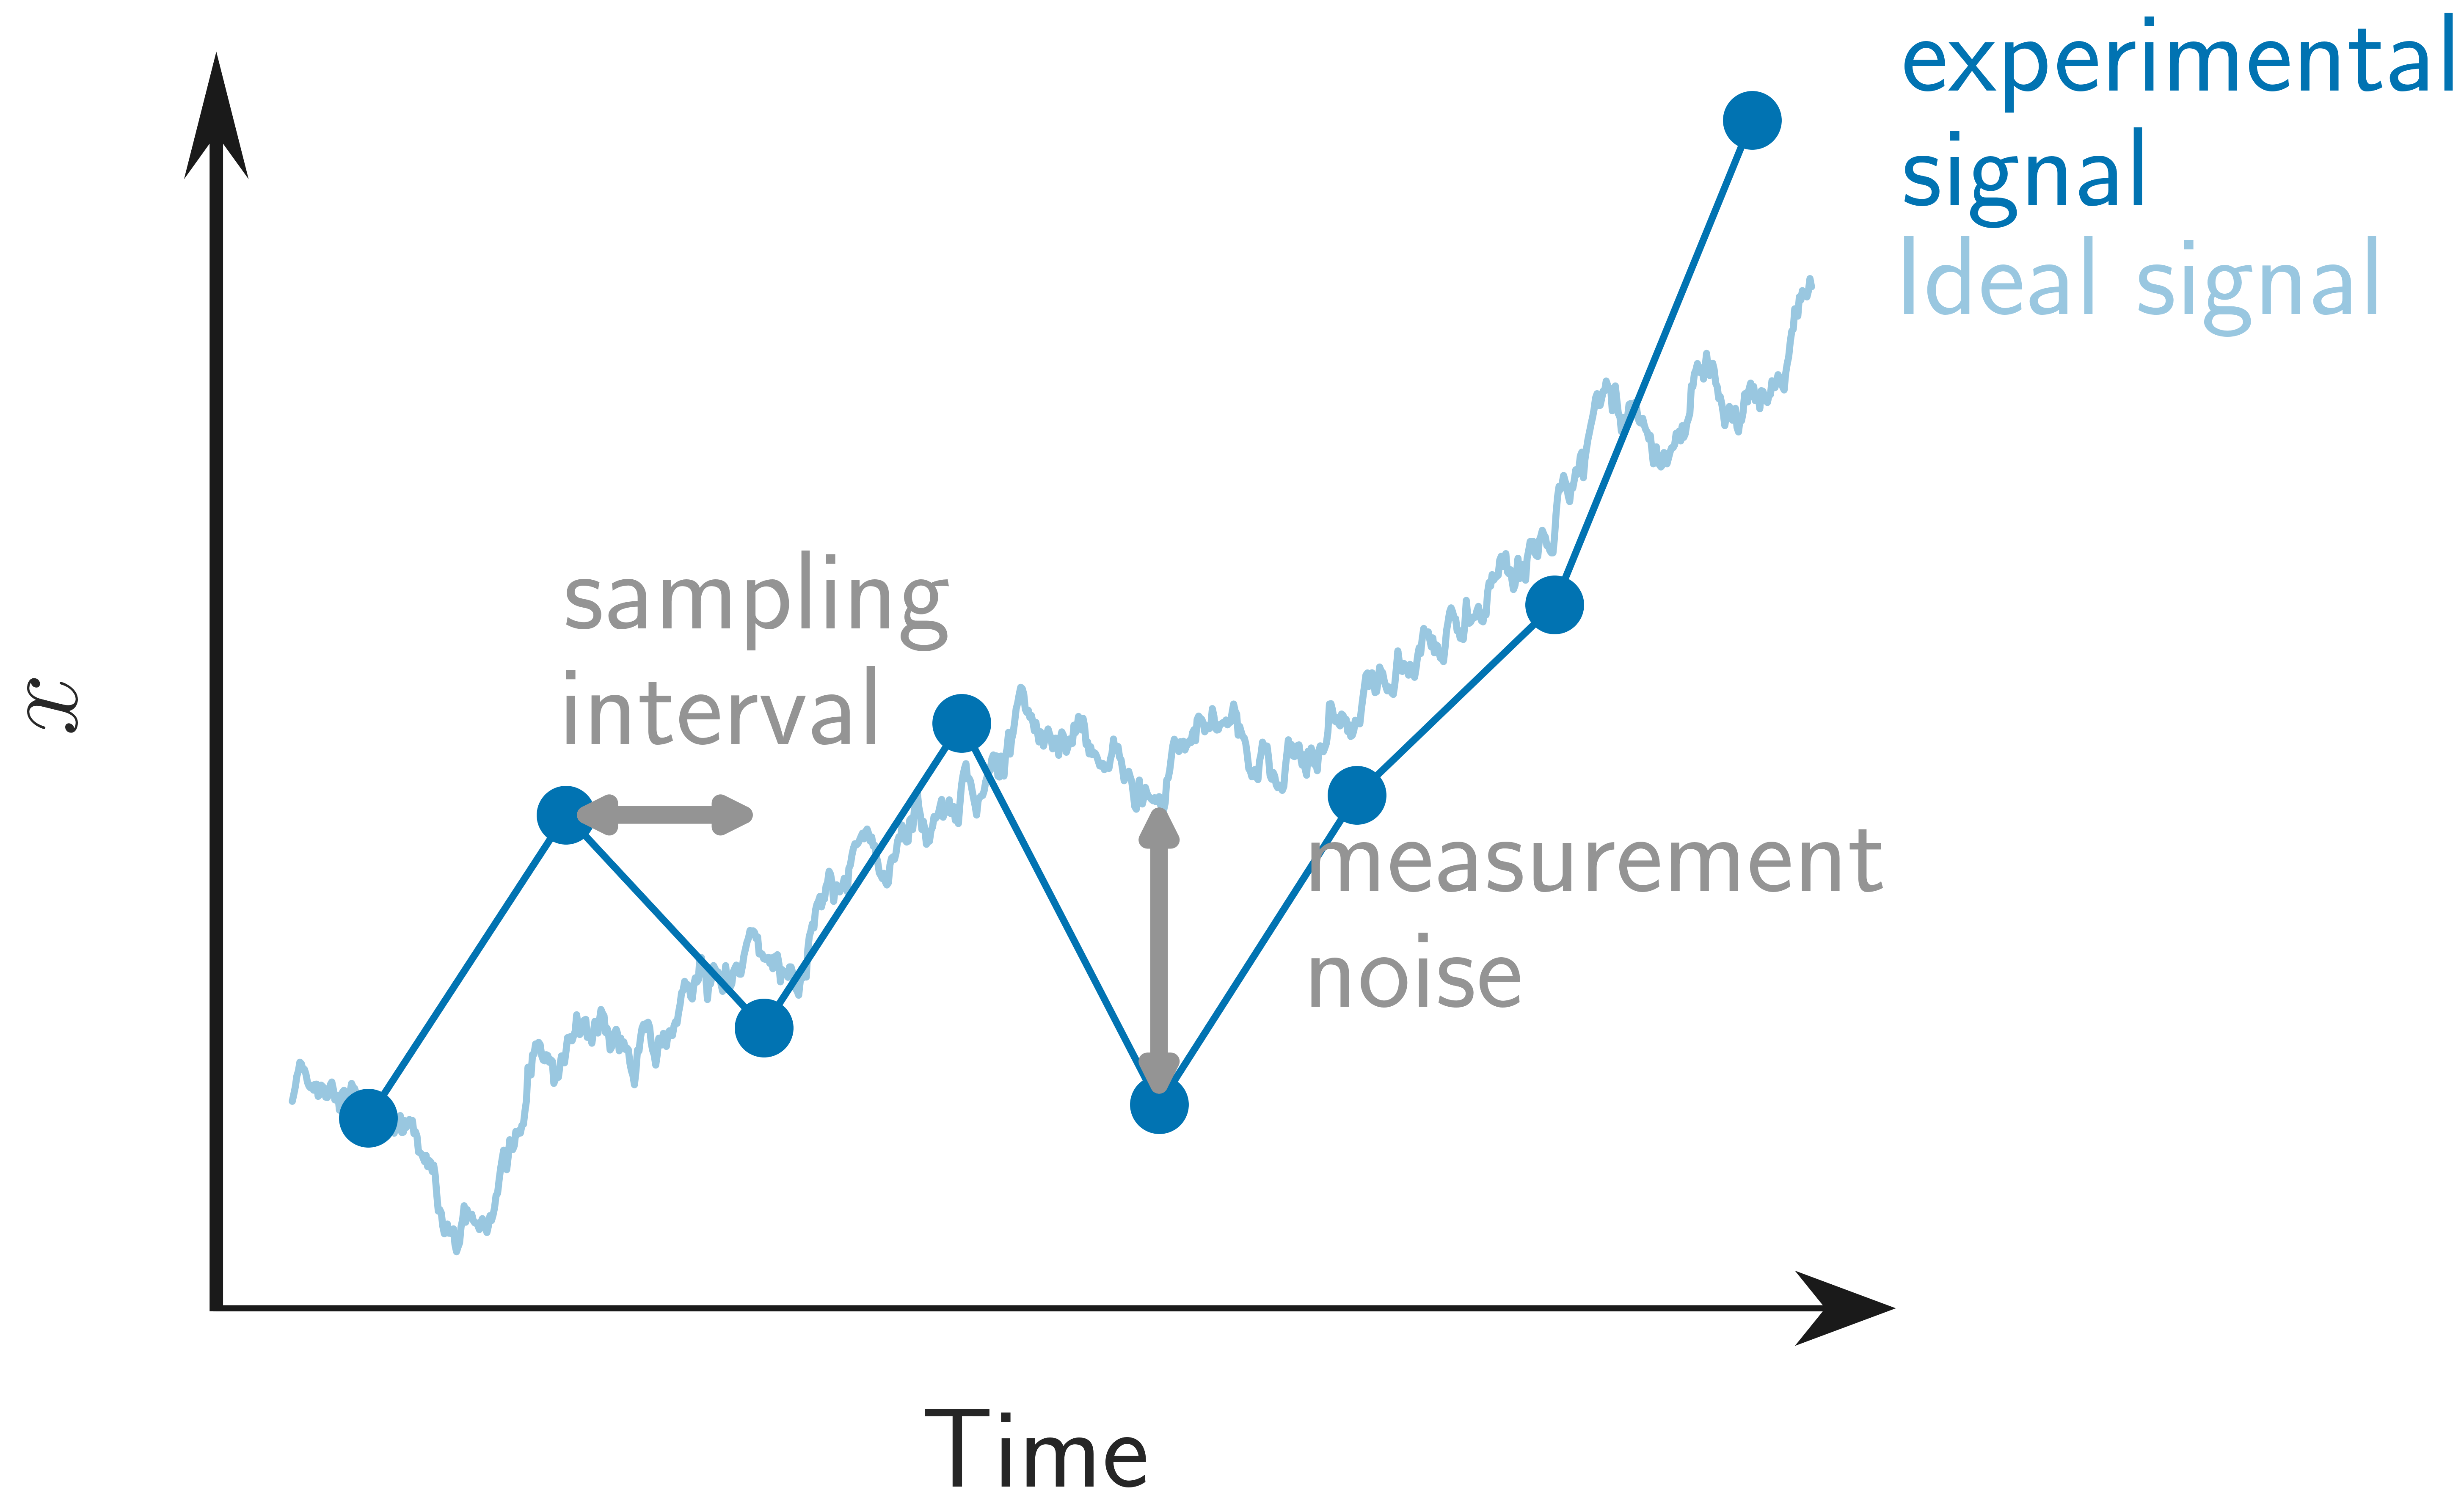
\includegraphics[width=0.5\linewidth]{fig/illustration_signal_2.png}
    \caption{Schema of the measured expiremental signal versus the real signal, which is impacted by sampling interval and measurement noise.}
    \label{fig:enter-label}
\end{figure}

\section{Robustness with Large Sampling Intervals}
In the previous chapter, we derived an estimator for the drift that uses the assumption $\frac{\Delta \bm{x_t}}{\Delta t} \approx \bm{f}(\bm{x_t})$ which relies on the sampling interval $\Delta t \to 0$. What is going to happen to the drift estimator if $\Delta t \to 0$ ? To answer this question, we need to take a look at 
\begin{equation}
    \frac{\Delta\bm{x_t}}{\Delta t} = \frac{1}{\Delta t}\int_t^{t+\Delta t} \left(\bm{f}(\bm{x_{t'}}) + \bm{\xi_{t'}} \right)\dd{t'}
    \label{eq:delta_x}
\end{equation}. To understand its behavior when $\Delta t$ increases, we Taylor expand $\bm{f}(\bm{x_{t'}})$ around $\bm{x_t}$ :
\begin{align}
    \bm{f}(\bm{x_{t'}}) &= \bm{f}(\bm{x_t}) + (\bm{x_t'} - \bm{x_{t}}).\nabla \bm{f}(\bm{x_t}) + \bm{D(x_t)}.\nabla^2\bm{f}(\bm{x_t}) (t'-t) + O(\Delta t^2) + O_\text{fluc}(\Delta t^{3/2})\\
    &= \bm{f}(\bm{x_t}) + \underbrace{\left(\bm{f}(\bm{x_t}).\nabla \bm{f}(\bm{x_t}) + \bm{D(x_t)}.\nabla^2\bm{f}(\bm{x_t})\right)}_{\bm{A}} (t'-t)  +O(\Delta t^2) + O_\text{fluc}(\Delta t^{1/2})
    \label{eq:Taylor_b}
\end{align}
where $\bm{D(x_t)}.\nabla^2\bm{f}(\bm{x_t})  = \sum_{\beta, \gamma} D_{\beta\gamma}(\bm{x_t})\pdv{\bm{f}}{x_{\beta}}{x_{\gamma}}$ and $O_\text{fluc}(\Delta t^{3/2})$ contains fluctuating terms such as $\int_t^{t+\Delta t}\bm{f(x_{t'})} \dd{t'} \int_t^{t+\Delta t}\bm{\xi_{t'}} \dd{t'}$ and higher orders. Thus, a more appropriate formulation for large sampling interval is $\frac{\Delta\bm{x_t}}{\Delta t} = \bm{f}(\bm{x_t}) + \bm{A} \frac{\Delta t}{2} + O(\Delta t^2) + O_\text{fluc}(\Delta t^{-1/2})$. But, by choosing $t'= t + \Delta t$ in \Eq{eq:Taylor_b}, we realize that $\bm{A} \approx \frac{\bm{f}(\bm{x_{t+ \Delta t})} - \bm{f}(\bm{x_t)}}{\Delta t}$ which leads to :
\begin{equation}
    \frac{\Delta\bm{x_t}}{\Delta t} = \frac{\bm{f}(\bm{x_{t+\Delta t})} + \bm{f}(\bm{x_t)}}{2}  + O(\Delta t^2) + O_\text{fluc}(\Delta t^{-1/2})
    \label{eq:delta_x_trapeze}
\end{equation}
So finally, we demonstrated that the trapeze formulation works for SDE integral. Wouaahhh, amazing. The interesting thing is to leverage this knowledge to improve the robustness of our drift estimator. To do so, we suppose that there exists a function base $\mathcal{B} = \{\bm{b_i}\}_{i=1,n}$ where $\bm{f}$ can be decomposed on such that : $\bm{f}(\bm{x}) = \sum_i \alpha_i\bm{b}_i(\bm{x})$. By multiplying \Eq{eq:delta_x_trapeze} by $\bm{b_i} \frac{\bm{\bar{D}}^{-1}}{4}$ and averaging over time, we get a simple equation 
\begin{equation}
    \avg{\frac{\Delta\bm{x_t}}{\Delta t}\cdot \frac{\bm{\bar{D}}^{-1}}{4}\bm{b_i}(\bm{x_t)}} = \sum_j \underbrace{\avg{\frac{\bm{b_j(x_t)} + \bm{b_j(x_{t+\Delta t})}}{2} \cdot \bm{\bar{D}}^{-1}\bm{b_i(x_t)}}}_{\left(G_{\mathcal{B}}^{Tr}\right)_{ij}} \alpha_j 
    \label{eq:chap_1_alpha_trapeze}
\end{equation}
which we can invert to obtain the learned parameters $\hat{\alpha_i}^{Tr}$
\begin{equation}
    \hat{\alpha_i}^{Tr} = \sum_j \left(G_{\mathcal{B}}^{Tr}\right)^{-1}_{ij} \avg{\frac{\Delta\bm{x_t}}{\Delta t}\cdot \bm{\bar{D}}^{-1}\bm{b_j}(\bm{x_t)}}
\end{equation}
Note that this estimator doesn't derive from the maximization of a likelihood function but when $\Delta t \to 0$, $\hat{\alpha_i}^{Tr}\to \hat{\alpha_i}$ which is a likelihood estimator. From the previous derivation, we expect that the reconstructed drift with $\hat{\alpha}_i$ has an error in $O(\Delta t)$ but for the reconstructed drift with the trapeze formulation $\hat{\alpha_i}^{Tr}$ we expect to have an error in $O(\Delta t^2)$. Indeed, we observe this behavior in \Fig{fig:Lorenz_benchmark}. This work leads to co-publication in~\cite{amiriInferringGeometricalDynamics2024}. Note that, I discovered recently that another PhD student was working on the same question and obtained the same trapeze estimator but with a different demonstration in~\cite{wannerHigherOrderDrift2024}.

\begin{figure}
    \centering
    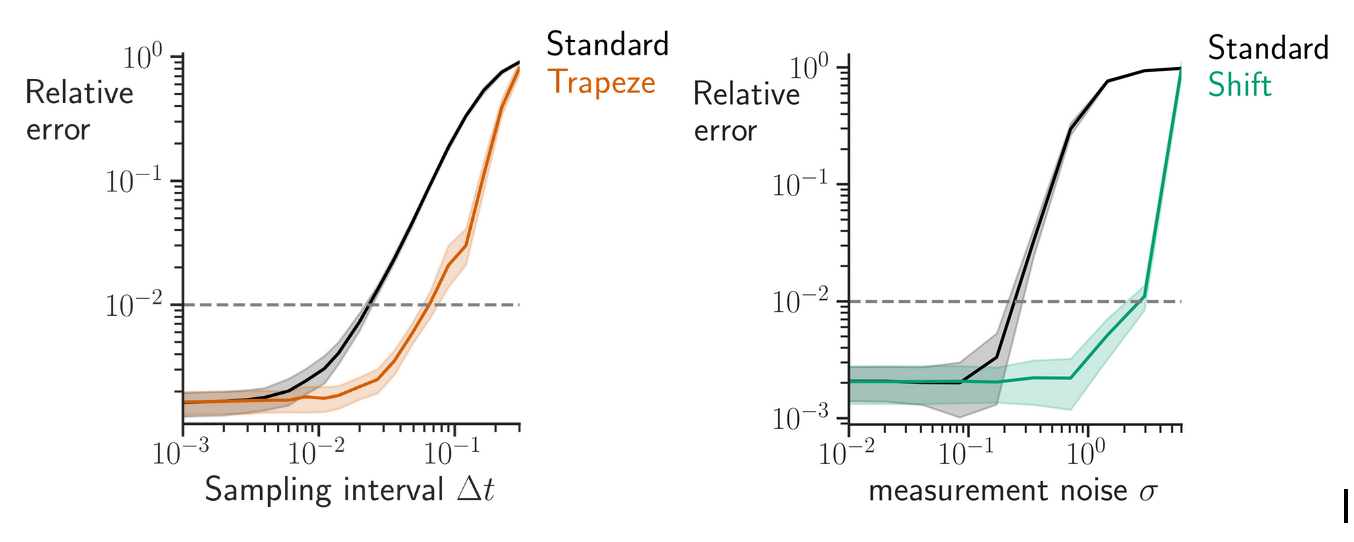
\includegraphics[width=0.5\linewidth]{fig/Lorenz_sampling_measurement noise_benchmark.png}
    \caption{NEED TO be done}
    \label{fig:Lorenz_benchmark}
\end{figure}












\section{Robustness Against Measurement Noise}

Measurement noise can be decomposed into two categories: the systematic error which always occurs with the same value (for instance, a wrongly calibrated balance), and the random error that varies from one observation to another. Here, we are only considering the random error by modeling the measurement noise as a Gaussian random variable which is added to the true trajectory $\bm{x_t} \rightarrow \bm{x_t} + \bm{\eta_t}$ with $\bm{\eta_t} \sim \mathcal{N}(0, \bm{\sigma})$. This simple measurement noise is going to affect our inferred drift. How ? Let us look at our estimator for the instantaneous drift $\frac{\Delta \bm{x_t}}{\Delta{t}} \rightarrow \frac{\Delta \bm{x_t}}{\Delta{t}} + \frac{\Delta \bm{\eta_t}}{\Delta{t}}$. From that, we see the dramatic coupling between the measurement noise and sampling interval: the standard deviation of the measurement noise is amplified by a prefactor $\frac{1}{\Delta t}$ which can be considerably big. Thus, when we infer the drift using the average : 
\begin{equation}
    \avg{\left(\frac{\Delta \bm{x_t}}{\Delta{t}} + \frac{\Delta \bm{\eta_t}}{\Delta{t}}\right)\cdot \frac{\bm{\bar{D}}^{-1}}{4}\bm{b_j}\left(\bm{x_t + \eta_t}\right)} = \avg{\frac{\Delta \bm{x_t}}{\Delta{t}} \cdot \frac{\bm{\bar{D}}^{-1}}{4}\bm{b_j}\left(\bm{x_t + \eta_t}\right)} + \avg{\frac{\Delta \bm{\eta_t}}{\Delta{t}}\cdot \frac{\bm{\bar{D}}^{-1}}{4}\bm{b_j}\left(\bm{x_t + \eta_t}\right)}
\end{equation}
the term $\avg{\frac{\Delta \bm{\eta_t}}{\Delta{t}}\cdot \frac{\bm{\bar{D}}^{-1}}{4}\bm{b_j}\left(\bm{x_t + \eta_t}\right)}$ is of order $\frac{\sigma^2}{\Delta t}$ and it is going to strongly bias our inference. We need a way to ensure this term to average to zero. How can we do that ? One way is to average over $\bm{b_j}(\bm{x_{t-\Delta t}})$ instead of $\bm{b_j}(\bm{x_t})$. Thus, we obtain : 

\begin{multline*}
    \avg{\left(\frac{\Delta \bm{x_t}}{\Delta{t}} + \frac{\Delta \bm{\eta_t}}{\Delta{t}}\right)\cdot \frac{\bm{\bar{D}}^{-1}}{4}\bm{b_j}\left(\bm{x_{t-\Delta t} + \eta_{t-\Delta t}}\right)} = \avg{\frac{\Delta \bm{x_{t}}}{\Delta{t}} \cdot \frac{\bm{\bar{D}}^{-1}}{4}\bm{b_j}\left(\bm{x_{t-\Delta t} + \eta_{t-\Delta t}}\right)} \\
    + \avg{\frac{\Delta \bm{\eta_t}}{\Delta{t}}\cdot \frac{\bm{\bar{D}}^{-1}}{4}\bm{b_j}\left(\bm{x_{t-\Delta t} + \eta_{t-\Delta t}}\right)}
\end{multline*}


\section{Comparative Discussion of Both Techniques}
Evaluate the advantages, limitations, and optimal conditions for each method.


